% ============================================================
% Přehled funkcí (zkrácená verze; všechny funkce včetně toho, co se děje
% na pozadí, popisuje dokumentace aplikace: docs/02-funkce.md v repozitáři)
% ============================================================
\section{Přehled funkcí aplikace}\label{sec:funkce-aplikace}

Tento oddíl popisuje funkce, které plní požadavky z~kapitoly~\ref{kap:analyza-workflow}, tedy průběh zakázky od přijetí zařízení po vystavení dokladu. Přehled všech funkcí a~míst v~aplikaci, kde je uživatel najde, je v~tabulce~\ref{tab:funkce}. Podrobný popis každé funkce (k~čemu slouží, jak ji uživatel používá, co se děje na pozadí a~se kterými tabulkami pracuje) je součástí dokumentace aplikace\footnote{\url{https://github.com/MajkyyQ/BusinessManager/blob/main/docs/02-funkce.md}}.

\begin{longtable}{p{0.30\textwidth}p{0.60\textwidth}}
\caption{Přehled funkcí aplikace}\label{tab:funkce}\\
\hline \textbf{Funkce} & \textbf{Kde v aplikaci} \\ \hline\endfirsthead
\hline \textbf{Funkce} & \textbf{Kde v aplikaci} \\ \hline\endhead
Přijetí zakázky & Zakázky $\rightarrow$ Nová zakázka \\
Řízení stavu zakázky & detail zakázky, seznam zakázek (zobrazení kanban) \\
Evidence zákazníků a zařízení & Zákazníci, Zařízení (včetně historie oprav) \\
Fotografie a přílohy & detail zakázky \\
Práce a materiál & detail zakázky, Nastavení $\rightarrow$ Katalogy \\
Cenová nabídka, faktura a platby & detail zakázky, Dokumenty \\
Přijaté objednávky & detail zakázky, Dokumenty \\
Zakázkový list a výsledné dokumenty & detail zakázky, náhled dokumentu \\
Export faktury do ISDOC & náhled a detail faktury \\
Přijaté faktury & Dokumenty $\rightarrow$ Přijatá faktura z~ISDOC \\
Šablony dokumentů a číslování dokladů & Nastavení $\rightarrow$ Dokumenty \\
Pracovní plocha & úvodní stránka, detail zakázky \\
Kalendář & Kalendář \\
Vyhledávání & všechny formuláře a seznamy \\
Správa záznamů, zaměstnanci a oprávnění & Nastavení, administrace \\
Průvodce prvním spuštěním & po instalaci \\
Zálohování & Nastavení $\rightarrow$ Systém, skript \path{zaloha.bat} \\
První nastavení aplikace & Nastavení $\rightarrow$ První nastavení aplikace, pracovní plocha \\
Tmavý režim & přepínač v~horní liště \\
Historie změn & záložka Historie změn, Nastavení \\
\hline
\end{longtable}

\subsection{Přijetí zakázky}

Formulář \enquote{Nová zakázka} odpovídá dřívějšímu papírovému zakázkovému listu, a~proto jsou všechny údaje na jedné obrazovce v~pořadí, v~jakém je pracovník od zákazníka zjišťuje. Pracovník vyhledá zákazníka zadáním části jména, firmy, telefonu nebo IČO, a~pokud neexistuje, založí ho v~dialogovém okně bez opuštění formuláře. Stejně vybere nebo založí zařízení (nabízí se jen zařízení vybraného zákazníka) a~kontaktní osobu, zapíše popis závady a~nahraje fotografie. Po uložení aplikace v~jedné databázové transakci vytvoří zakázku se stavem \enquote{Nová}, přidělí jí číslo podle číselné řady, uloží navázané záznamy, zapíše událost do kalendáře a~záznam do historie změn.

\subsection{Řízení stavu zakázky}

Stav zakázky ukazuje, v~jaké fázi se oprava nachází, a~umožňuje rychle zjistit, která zařízení jsou ve firmě a~co je připraveno k~vyzvednutí. V~detailu zakázky se zobrazují jen tlačítka akcí, které jsou v~aktuálním stavu dovoleny (obrázek~\ref{fig:stavy}). Povolené přechody jsou v~kódu popsány dvěma slovníky (stav $\rightarrow$ povolené akce, akce $\rightarrow$ cílový stav) a~pohled akci před provedením ověří. Při vydání zařízení se uloží datum vydání a~kdo zařízení vydal. Ruční změnu stavu mimo pracovní postup smí jen administrátor nebo zaměstnanec s~oprávněním. Sám se stav mění jen u~nové zakázky: přidáním první práce přejde do stavu \enquote{Rozpracováno} a~vytvořením nabídky do stavu \enquote{Čeká na schválení}; obě změny se zapíší do historie. Každý stav má barvu, kterou si firma zvolí v~nastavení, a~vedle barvy je vždy uveden i~název stavu.

\begin{figure}[htbp]
\centering
\begin{tikzpicture}[font=\footnotesize\sffamily,
    st/.style={draw, rounded corners=6pt, fill=gray!8, minimum height=0.75cm, inner sep=3pt, align=center},
    akce/.style={font=\scriptsize\sffamily, inner sep=1.5pt}]
  \node[st] (nova) at (0,0) {Nová};
  \node[st] (schv) at (3.4,1.5) {Čeká na schválení};
  \node[st] (dil) at (3.4,-1.5) {Čeká na díl};
  \node[st] (roz) at (6.6,0) {Rozpracováno};
  \node[st] (opr) at (10.0,0) {Opraveno};
  \node[st] (prip) at (13.3,0) {Připraveno\\k vyzvednutí};
  \node[st] (vyd) at (13.3,-2.2) {Vydáno};
  \node[st] (zrus) at (0,-2.2) {Zrušeno};
  \draw[bm sipka] (nova) -- node[akce, above] {zahájit} (roz);
  \draw[bm sipka] (nova) -- (schv);
  \draw[bm sipka] (nova) -- (dil);
  \draw[bm sipka] (schv) -- node[akce, above, sloped, pos=0.6] {schváleno} (roz);
  \draw[bm sipka] (dil) -- node[akce, below, sloped, pos=0.6] {díl dorazil} (roz);
  \draw[bm sipka] (roz) -- node[akce, above] {dokončit} (opr);
  \draw[bm sipka] (opr) -- node[akce, above] {připravit} (prip);
  \draw[bm sipka] (prip) -- node[akce, right] {vydat} (vyd);
  \draw[bm sipka] ([xshift=-2mm]nova.south) -- node[akce, left] {zrušit} ([xshift=-2mm]zrus.north);
  \draw[bm sipka, densely dashed] ([xshift=2mm]zrus.north) -- node[akce, right] {obnovit} ([xshift=2mm]nova.south);
  \draw[bm sipka, densely dashed] (vyd.west) -- node[akce, above] {znovu otevřít} (vyd.west -| roz.south) -- (roz.south);
\end{tikzpicture}
\caption{Hlavní přechody mezi stavy zakázky (zrušit lze i rozpracovanou zakázku a z rozpracované zakázky lze přejít zpět do čekání)}\label{fig:stavy}
\end{figure}

\subsection{Práce a materiál}

Evidence provedených prací a~použitého materiálu je podkladem pro ocenění zakázky a~pro položky dokladů. U~práce uživatel vybere typ úkonu z~katalogu, zadá cenu, sazbu DPH a~pracovníky. Materiál vyhledá v~katalogu a~zadá množství; aplikace sama doplní poslední známou cenu a~při uložení ji k~zakázce \enquote{zamrazí}, takže změna ceníku neovlivní starší zakázky. Tlačítkem \enquote{+ Přidat} lze do jednoho formuláře zapsat více prací nebo položek materiálu a~uložit je najednou. Poznámka k~práci je interní a~do zakázkového listu ani do položek dokladu se nepropisuje.

\subsection{Cenová nabídka, faktura a platby}

Nabídka i~faktura se vytvoří z~pracovní plochy zakázky. Formulář ukáže náhled položek, které budou převzaty, včetně součtů. Každá práce se stane položkou s~množstvím 1, každý materiál položkou s~množstvím, jednotkou a~cenou; chybějící sazbu DPH doplní výchozí sazba firmy. Položky vznikají jen ze zakázky, ručně se do vystaveného dokladu nepřidávají. Doklad dostane číslo podle číselné řady, kterou si firma nastaví podle vzoru (například \texttt{Fa0001} nebo \texttt{001-04-11/2026}), a~uloží si kopii údajů zákazníka. Nabídka přebírá pořadové číslo zakázky, další nabídka ke stejné zakázce dostane příponu (například \texttt{2026-048-2}). Po vytvoření nabídky aplikace nabídne pokračovat do zakázky nebo rovnou na fakturu. Spolu s~fakturou se založí platba ve stavu \enquote{Čeká na zaplacení}, kterou uživatel po úhradě jedním tlačítkem označí jako zaplacenou; obě události se zapíší do kalendáře.

Zákazník může zaplatit i~přímo při vyzvednutí zařízení bez faktury, typicky jen poplatek za diagnostiku, když se zařízení neopravuje. Tlačítko \enquote{Vydat zákazníkovi} proto otevře okno se dvěma volbami (obrázek~\ref{obr:bm-platba-na-miste}). Při volbě \enquote{Zaplaceno na místě bez faktury} uživatel potvrdí částku (předvyplní se součet práce a~materiálu s~DPH), zvolí způsob platby (hotově, QR kódem nebo kartou) a~může doplnit poznámku. Aplikace pak v~jedné databázové transakci založí platbu ve stavu \enquote{Zaplaceno} navázanou jen na zakázku a~zakázku vydá. Platba se zapíše do historie zakázky i~do kalendáře a~na pracovní ploše zakázky se zobrazí u~stavu. Volba \enquote{Bez platby na místě} slouží pro placení fakturou, záruční opravu nebo opravu zdarma. U~vydané zakázky bez faktury lze platbu zapsat i~dodatečně.

\begin{figure}[H]
\centering
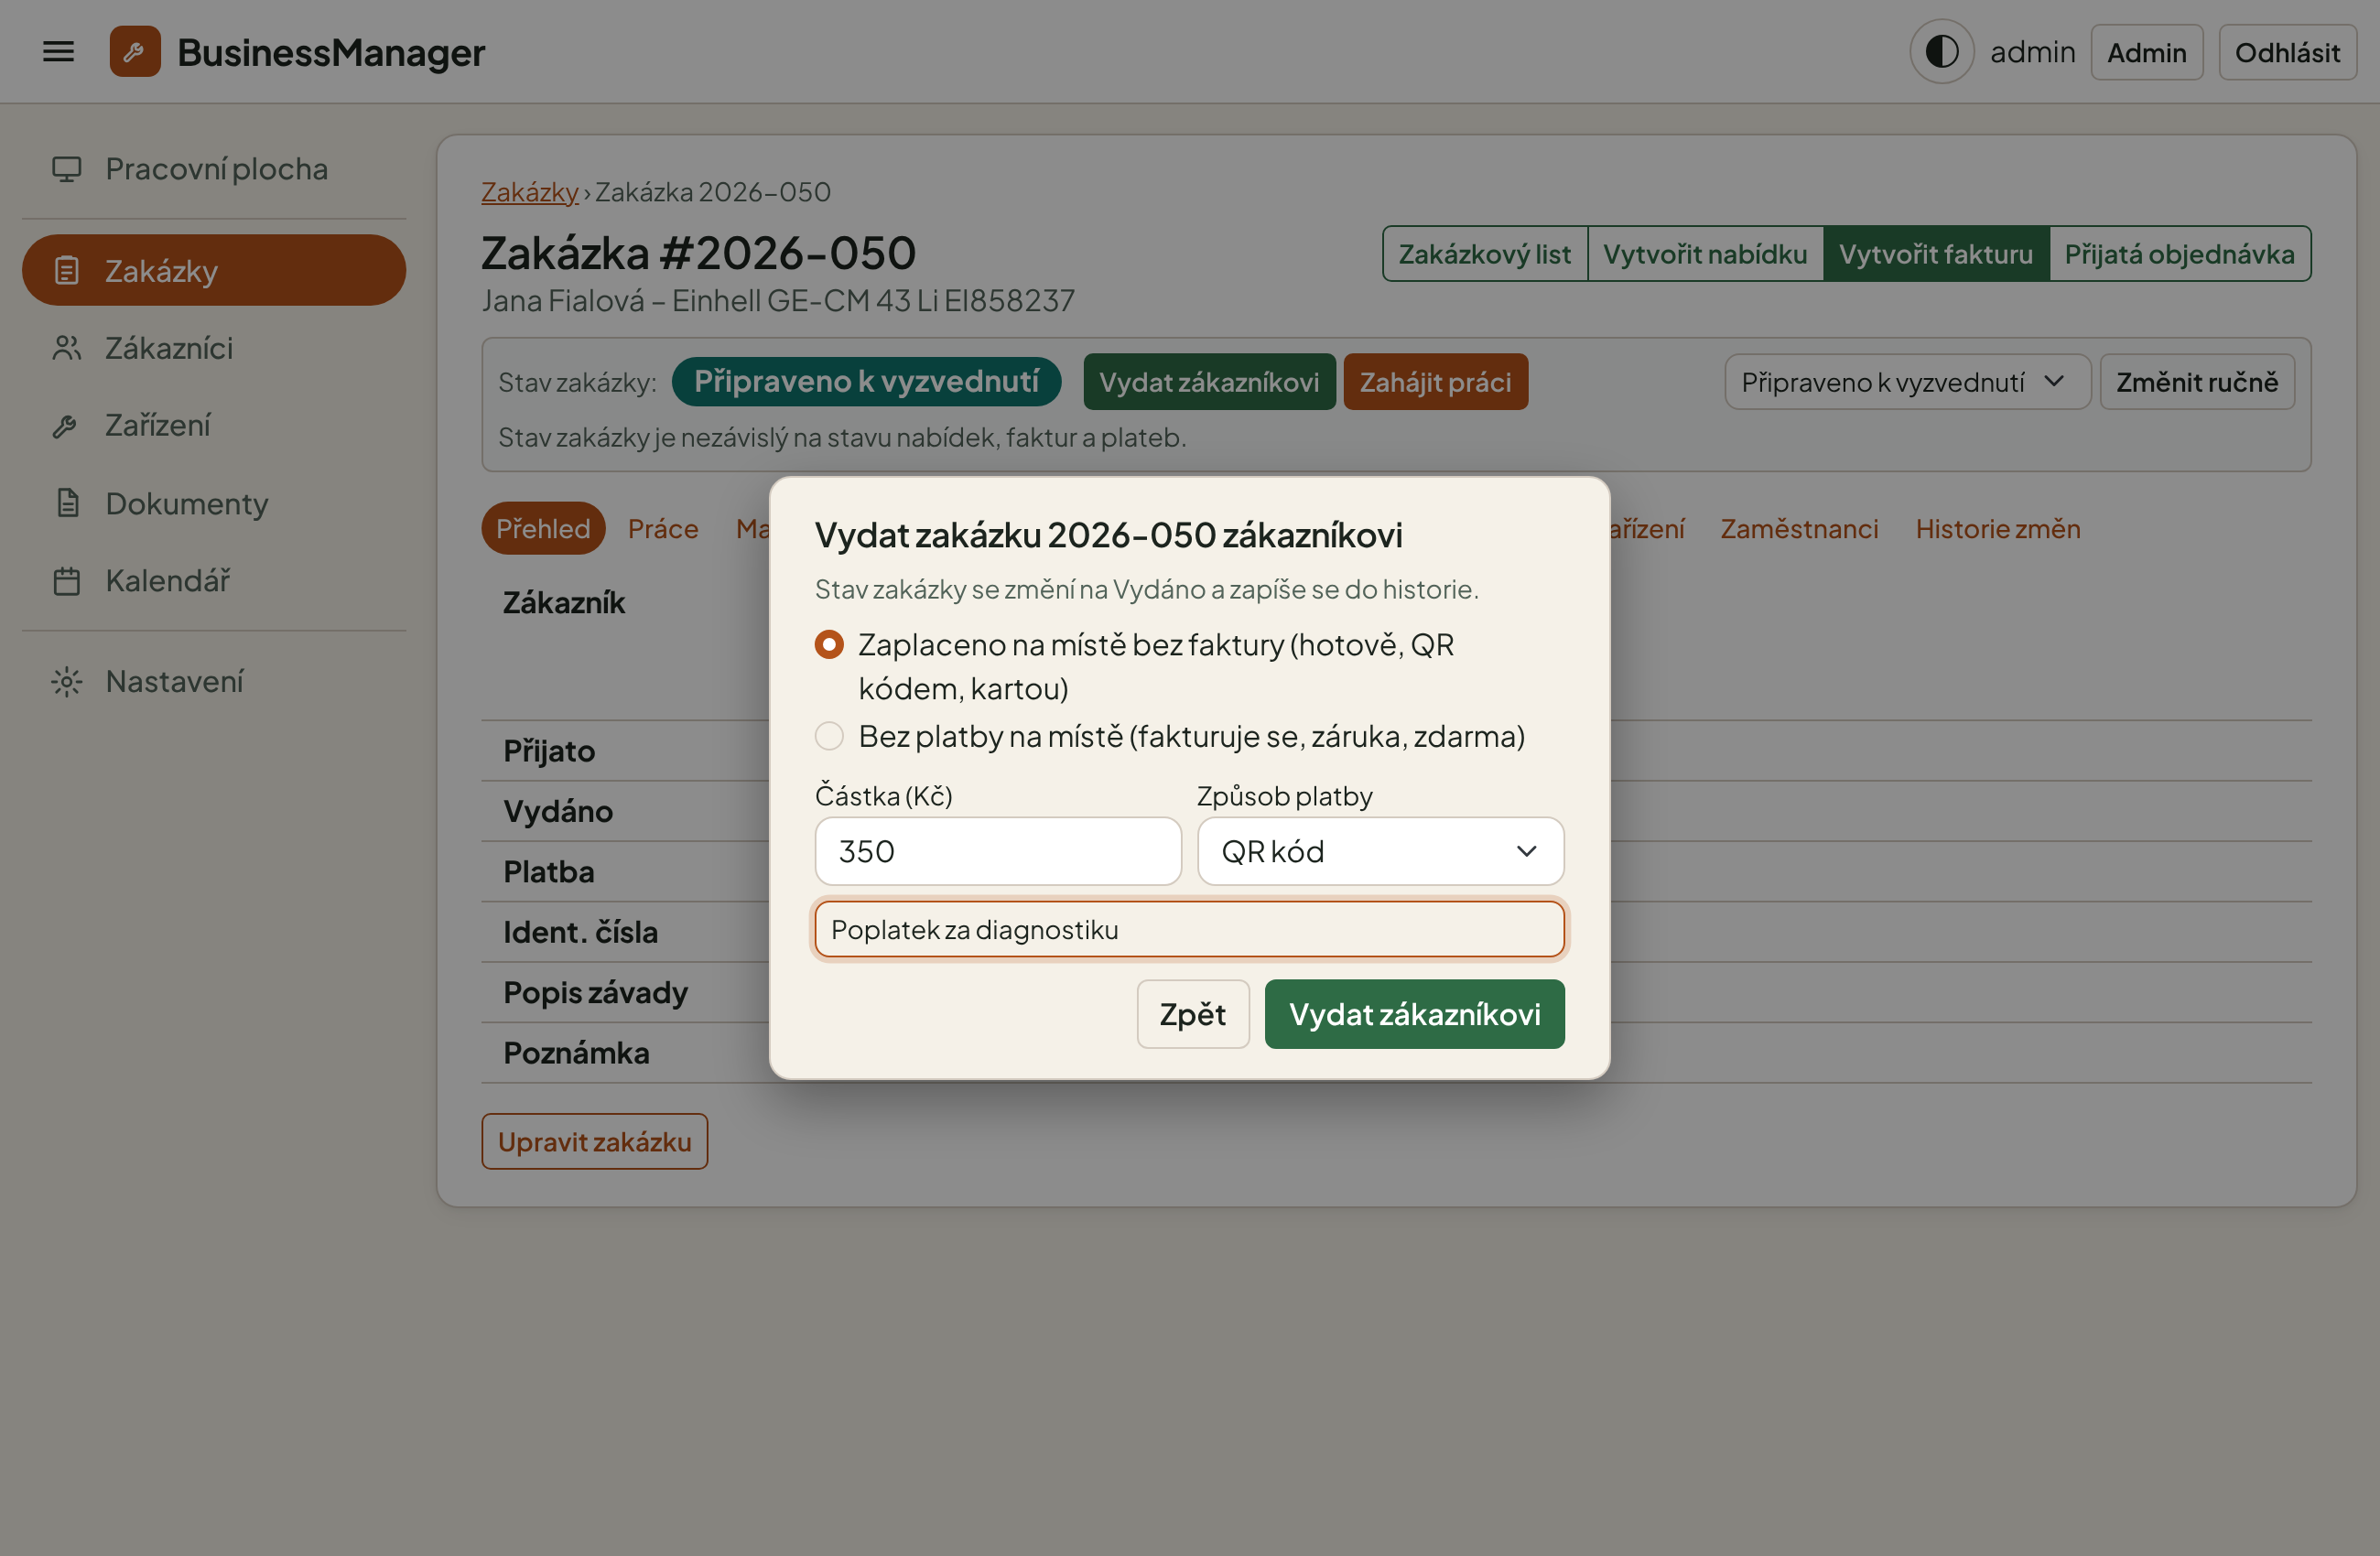
\includegraphics[width=\linewidth]{obrazky/navrh/bm-vydat-zaplaceno-na-miste.png}
\caption{Vydání zakázky se zápisem platby na místě bez faktury (zdroj: vlastní)}\label{obr:bm-platba-na-miste}
\end{figure}

Jak se data zakázky převedou na doklad a~dále na dokument, popisuje oddíl~\ref{sec:tok-dat}.

\subsection{Výsledné dokumenty}

Zakázkový list, nabídku i~fakturu lze zobrazit v~náhledu, vytisknout nebo stáhnout jako PDF s~názvem podle firemních zvyklostí. Volba \enquote{Změnit šablonu} zobrazí miniatury všech šablon daného typu a~kliknutím se dokument zobrazí v~jiné šabloně. Fakturu lze stáhnout i~jako elektronickou fakturu ISDOC. Systém šablon popisuje oddíl~\ref{sec:sablony}.

\subsection{Přijaté faktury a kalendář}\label{sec:prijate-faktury}

Faktury od dodavatelů uživatel nahraje jako soubor ISDOC. Aplikace z~něj přečte údaje faktury a~dodavatele, dodavatele dohledá v~evidenci nebo založí, upozorní na duplicitní fakturu a~uloží záznam s~původním souborem. Do kalendáře se zapíše doručení, splatnost a~po úhradě i~zaplacení. Fakturu, která přišla jen na papíře, lze zadat ručně.

Kalendář sdružuje automatické události (přijetí a~vydání zakázek, vystavení a~zaplacení faktur, splatnost přijatých faktur) s~ručně zadanými termíny. Lze ho zobrazit po měsících, týdnech nebo dnech a~filtrovat podle typu události a~zaměstnance. V~měsíčním zobrazení se u~dne ukážou nejvýše tři události, kliknutím na den se otevře okno se všemi událostmi dne. Vlastní událost lze rychle přidat tlačítkem \enquote{+} přímo u~dne.
